%%%%%%%%%%%%%%%%%%%%%%%%%%%%%%%%%%%%%%%%%%%%%%%%%%%%%%%%%%%%%%%%%%%%%%%%%
% ARTICLE ABOUT FATE OF SYNONYMOUS MUTATIONS IN HIV
%%%%%%%%%%%%%%%%%%%%%%%%%%%%%%%%%%%%%%%%%%%%%%%%%%%%%%%%%%%%%%%%%%%%%%%%%
%\documentclass[pre, onecolumn, preprint]{revtex}
\documentclass[11pt]{article}
%%%%%%%%%%%%%%%%%%%%%%%%%%%%%%%%%%%%%%%%%%%%%%%%%%%%%%%%%%%%%%%%%%%%%%%%%
%%%%%%%%%%%%%%%%%%%%%%%%%%%%%%%%%%%%%%%%%%%%%%%%%%%%%%%%%%%%%%%%%%%%%%%%%
\usepackage[english]{babel}
\usepackage[utf8x]{inputenc}
\usepackage{amsmath,amsfonts,amssymb,eucal,eurosym,textcomp}
\usepackage{color}
\usepackage{graphicx}
\usepackage[caption=false]{subfig}
\usepackage[numbers]{natbib}
\usepackage{pslatex}
\usepackage{lineno}
\linenumbers

%%%%%%%%%%%%%%%%%%%%%%%%%%%%%%%%%%%%%%%%%%%%%%%%%%%%%%%%%%%%%%%%%%%%%%%%%
\graphicspath{{./figures/}}
%%%%%%%%%%%%%%%%%%%%%%%%%%%%%%%%%%%%%%%%%%%%%%%%%%%%%%%%%%%%%%%%%%%%%%%%%
\newcommand{\comment}[1]{\textit{\textcolor{red}{#1}}}
\newcommand{\mut}{\mu}
\newcommand{\mfit}{\langle F\rangle}
\newcommand{\mexpfit}{\langle e^{F}\rangle}
\newcommand{\pfix}{P_{\mathrm{fix}}}
\newcommand{\ox}{r}
\newcommand{\co}{\rho}
\newcommand{\gt}{g}
\newcommand{\locus}{s}
\newcommand{\locuspm}{t}
\newcommand{\OO}{\mathcal{O}}
\newcommand{\FIG}[1]{Fig.~\ref{fig:#1}}
\newcommand{\FIGS}[2]{Figs.~\ref{fig:#1} and~\ref{fig:#2}}
\newcommand{\env}{\textit{env}}
\newcommand{\rev}{\textit{rev}}
\newcommand{\pol}{\textit{pol}}
\newcommand{\shankaregion}{C2-V5}
\newcommand{\PCApat}{1}
\newcommand{\syndiv}{2}
\newcommand{\timedependence}{3}
\newcommand{\withinepi}{4}
%%%%%%%%%%%%%%%%%%%%%%%%%%%%%%%%%%%%%%%%%%%%%%%%%%%%%%%%%%%%%%%%%%%%%%%%%
\renewcommand{\thesubfigure}{\Alph{subfigure}}
\newcommand{\Author}{Fabio~Zanini and Richard~A.~Neher}
\newcommand{\Title}{Quantifying selection against synonymous mutations in HIV-1 \env{} evolution}
\newcommand{\Affiliation}{Max Planck Institute for Developmental Biology, 72076 T\"ubingen, Germany}
\newcommand{\Keywords}{{HIV}, {synonymous}, {population genetics}}
%%%%%%%%%%%%%%%%%%%%%%%%%%%%%%%%%%%%%%%%%%%%%%%%%%%%%%%%%%%%%%%%%%%%%%%%%
\usepackage{hyperref}
\hypersetup{colorlinks,linkcolor=red,citecolor=blue, pdfauthor={\Author}, pdftitle={\Title}, pdfkeywords={\Keywords}}
%%%%%%%%%%%%%%%%%%%%%%%%%%%%%%%%%%%%%%%%%%%%%%%%%%%%%%%%%%%%%%%%%%%%%%%%%
\linespread{1.5}
\begin{document}
\title{\Title}
\author{\Author\\ \Affiliation}
%\affiliation{\Affiliation}
\date{\today}
%%%%%%%%%%%%%%%%%%%%%%%%%%%%%%%%%%%%%%%%%%%%%%%%%%%%%%%%%%%%%%%%%%%%%%%%%
\maketitle

\newpage
%\begin{abstract}
\section*{Abstract}
\noindent
Intrapatient HIV-1 evolution is driven by the adaptive immune system
resulting in rapid change of HIV-1 proteins. When cytotoxic CD8${}^+$ T-cells
or neutralizing antibodies target a new epitope, the virus often escapes via
nonsynonymous mutations that impair recognition. Synonymous mutations do not
affect this interplay and are often assumed to be neutral. We test this
assumption by tracking  synonymous mutations in 
longitudinal intrapatient data from the \shankaregion{} part of the \env{}
gene. We find that most synonymous variants are lost even though
they often reach high frequencies in the viral population, suggesting a
cost to the virus. Using published data
from SHAPE assays, we find that synonymous mutations that disrupt base pairs
in RNA stems flanking the variable loops of gp120 are more likely to be lost than other
synonymous changes: these RNA hairpins might be important for HIV-1.
Computational modeling indicates that (i) most synonymous mutations in this
genomic region have a selection coefficient of the order of $-0.002$, and
(ii) synonymous variants rise to high frequency by genetic hitchhiking on neighboring beneficial
variants. This weak selection against synonymous substitutions does not
result in a strong pattern of conservation in cross sectional data, but
slows down the rate of evolution considerably. Our findings are consistent with the
notion that large scale patterns of RNA structure are functionally
relevant, while the precise base pairing pattern is not.
%\end{abstract}
%%%%%%%%%%%%%%%%%%%%%%%%%%%%%%%%%%%%%%%%%%%%%%%%%%%%%%%%%%%%%%%%%%%%%%%%%
%%%%%%%%%%%%%%%%%%%%%%%%%%%%%%%%%%%%%%%%%%%%%%%%%%%%%%%%%%%%%%%%%%%%%%%%%
\section*{Introduction}
%%%%%%%%%%%%%%%%%%%%%%%%%%%%%%%%%%%%%%%%%%%%%%%%%%%%%%%%%%%%%%%%%%%%%%%%%
HIV-1 evolves rapidly within a single host during the course of the infection.
This evolution is driven by strong selection imposed by the host immune system
via cytotoxic CD8${}^+$ T-cells (CTLs) and neutralizing antibodies
(nAbs)~\citep{rambaut_causes_2004} and facilitated by HIV-1's high mutation rate
~\citep{mansky_lower_1995,abram_nature_2010}. Escape mutations
in epitopes targeted by CTLs are typically observed during early infection and spread
rapidly through the population~\citep{mcmichael_immune_2009}. During chronic
infection, the most rapidly evolving parts of the HIV-1 genome are the variable
loops V1-V5 in the envelope protein gp120 (V loops), which change to avoid recognition by
nAbs. Escape mutations in \env{}, the gene encoding gp120, spread through the
viral population within a few months.
Consistent with this time scale, it is found that serum from a particular time
typically neutralizes autologous virus extracted more than 3-6 months earlier but not contemporary
virus \citep{richman_rapid_2003}.

Escape mutations are selected because they change the amino acid sequence of
viral proteins in a way that reduces antibody binding or epitope presentation.
Conversely, synonymous mutations do not modify the viral proteins and are
commonly used as approximately neutral markers in studies of viral evolution,
i.e., as a negative control for detecting selected
sites \citep{Bhatt:2011p43255,Hurst:2002p32608,Chen:2004p22606}. In addition to
maintaining protein function and avoiding the adaptive immune recognition,
however, the HIV-1 genome has to ensure efficient processing and translation,
nuclear export, and packaging into the viral capsid: all these processes operate
at the RNA level and are sensitive to synonymous changes. Several
important RNA secondary structures have been characterized in detail, including the HIV-1
\rev{} response element (RRE) in \env{} which enhances nuclear export of full length
or partially spliced viral transcripts via a complex hairpin RNA structure
\citep{fernandes_hiv-1_2012}. In fact, the HIV-1 genome is full of RNA
structures \citep{watts_architecture_2009} with no or unknown
function. However, large scale modification of secondary structures
can results in substantial reduction of the replication capacity
\citep{keating_rich_2009} and the propensity of forming RNA stems
anticorrelates with the rate of evolution
\citep{forsdyke_reciprocal_1995,snoeck_mapping_2011}. 
These poorly characterized RNA structures are conserved to varying degree between HIV-1 and
SIV: corresponding regions tend to be part
of similar structural elements, but individual base pairings are very
rarely conserved \citep{pollom_comparison_2013}. 

In this paper, we characterize the dynamics of synonymous mutations in \env{}
and show that, in the region of the V loops, a large fraction of these mutations
is deleterious. Despite their fitness cost, deleterious synonymous variants
rise in frequency in the viral population via genetic hitchhiking due to limited
recombination in HIV-1 populations~\citep{neher_recombination_2010,
batorsky_estimate_2011}. We show a strong correlation between the fate of a
synonymous variant and the surrounding RNA structure. We then compare our
observations to computational models and obtain estimates for the effect of
synonymous mutations on viral fitness.

%%%%%%%%%%%%%%%%%%%%%%%%%%%%%%%%%%%%%%%%%%%%%%%%%%%%%%%%%%%%%%%%%%%%%%%%%
\section*{Materials \& Methods}
%%%%%%%%%%%%%%%%%%%%%%%%%%%%%%%%%%%%%%%%%%%%%%%%%%%%%%%%%%%%%%%%%%%%%%%%%
\subsection*{Sequence data collection}
%%%%%%%%%%%%%%%%%%%%%%%%%%%%%%%%%%%%%%%%%%%%%%%%%%%%%%%%%%%%%%%%%%%%%%%%%
Longitudinal intrapatient viral RNA sequences were collected from published
studies \citep{shankarappa_consistent_1999, liu_selection_2006,
bunnik_autologous_2008} and downloaded from the Los Alamos National Laboratory
(LANL) HIV sequence database~\citep{LANL2012}. Some patients
show substantial population structure and were excluded (see
\figurename~S\PCApat); a total of 11 patients with 4-23 time points each and
approximately 10 sequences per time point were analyzed. The time intervals
between two consecutive sequences ranged from 1 to 34 months, most of them
between 6 and 10 months.

%%%%%%%%%%%%%%%%%%%%%%%%%%%%%%%%%%%%%%%%%%%%%%%%%%%%%%%%%%%%%%%%%%%%%%%%%
\subsection*{Sequence analysis}
%%%%%%%%%%%%%%%%%%%%%%%%%%%%%%%%%%%%%%%%%%%%%%%%%%%%%%%%%%%%%%%%%%%%%%%%%
The sequences were translated and the resulting amino acid sequences aligned
using Muscle~\citep{edgar_muscle:_2004} to each other and the NL4-3 reference
sequence separately for each patient. Within each patient, the consensus
nucleotide sequence at the first time point was used to classify alleles as
``ancestral'' or ``derived'' at all sites. Sites that include large
frequencies of gaps were excluded from the analysis to avoid artifactual
substitutions due to alignment errors. Allele frequencies at different time
points were extracted from the multiple sequence alignment.

A mutation was considered synonymous if it did not change the amino acid
corresponding to the codon, and if the rest of the codon was in the ancestral
state. Codons with more than one mutation were discarded. Slightly different
criteria for synonymous/nonsynonymous discrimination yielded similar results.

%%%%%%%%%%%%%%%%%%%%%%%%%%%%%%%%%%%%%%%%%%%%%%%%%%%%%%%%%%%%%%%%%%%%%%%%%
\subsection*{Fixation probability and secondary structure}
%%%%%%%%%%%%%%%%%%%%%%%%%%%%%%%%%%%%%%%%%%%%%%%%%%%%%%%%%%%%%%%%%%%%%%%%%
For the estimates of time to fixation/extinction, SNVs were binned by
frequency and the time to first reaching either fixation or extinction was
stored. The fixation probability was determined as the long-time limit of the
resulting curves. Mutations that reached high frequency but neither fixed nor
were lost were classified as ``floating'', with one exception: if they first
reached high frequencies within 3 years of the last time point, it was assumed
they had not had sufficient time to settle, so they were discarded.

The SHAPE scores quantifying the degree of base pairing of individuals sites in
the HIV-1 genome were downloaded from the journal website
\citep{watts_architecture_2009}. Wherever possible, SHAPE reactivities were
assigned to sites in the multiple sequence alignments for each patient through
the alignment to the sequence of the NL4-3 virus used in
\citep{watts_architecture_2009}. Problematic assignments in indel-rich
regions were excluded from the analysis. The variable loops and flanking
regions were identified manually starting from the annotated reference HXB2
sequence from the LANL HIV database~\citep{LANL2012}. 

%%%%%%%%%%%%%%%%%%%%%%%%%%%%%%%%%%%%%%%%%%%%%%%%%%%%%%%%%%%%%%%%%%%%%%%%%
\subsection*{Computer simulations}
%%%%%%%%%%%%%%%%%%%%%%%%%%%%%%%%%%%%%%%%%%%%%%%%%%%%%%%%%%%%%%%%%%%%%%%%%
Computer simulations were performed using FFPopSim
\citep{zanini_ffpopsim:_2012}. Briefly, FFPopSim enables individual-based
simulations where each site in the genome is represented by one bit that can be
in one of two states. Outcrossing rates, crossover rates, mutations rates and
arbitrary fitness functions can be specified. We used a generation time of 1
day, an outcrossing rate of $r=0.01$ per day \citep{batorsky_estimate_2011,
neher_recombination_2010}, a mutation rate of $\mu=10^{-5}$
\citep{mansky_lower_1995, abram_nature_2010} and simulated intrapatient
evolution for 6000 days. For simplicity, third positions of every codon were
deemed synonymous and assigned either a selection coefficient $0$ with
probability $1-\alpha$ or a deleterious effect $s_d$ with probability $\alpha$.
Mutations at the first and second positions were assigned strongly deleterious 
fitness effects 0.02. At 
rate $k_A$, a random locus in the genome is designated an epitope that can
escape by one or several mutations with exponentially distributed escape rates
with mean $\epsilon$. Both full-length HIV-1 genomes and \env{}-only simulations
were performed and yielded comparable results.

The simulations were repeated 2400 times with random choices for the following
parameters: the fraction of deleterious sites $\alpha$ was sampled uniformly
between 0.75 and 1.0; the average deleterious effect $s_d$ was sampled such that
its logarithm was uniformly distributed  between $10^{-4}$ and $10^{-2}$; the
average escape rate $\epsilon$ of escape mutation was sampled such that its logarithm was
uniform between $10^{-2.5}$ and $10^{-1.5}$ and the rate $k_A$ of new antibody
challenges such that its logarithm was uniform between $10^{-3}$ and $10^{-2}$
per generation. Populations were initialized with a homogeneous founder
population and were kept at an average size of $N=10^4$ throughout the
simulation. After 30 generations of burn-in to create genetic diversity, new
epitopes were introduced at a constant rate $k_A$. 

For the models with competition within epitopes, a complex epistatic fitness
landscape was designed such that each single mutant is sufficient for full
escape. Specifically, each mutation has an additive effect equal to the
escape rate, but interacts with all other escape mutations in the same
epitope with a negative effect of the same magnitude. 
Higher order terms were included to make sure that not
only double mutants, but all k-mutants with $k \geq 1$ had the same fitness (see
supplementary materials). To model recognition of escape variants by the
evolving immune system, the beneficial effect of an escape mutation was set
to its previous cost of -0.02 with a probability per generation proportional to
the frequency of the escape variant.

For each set of parameters, fixation probabilities and probabilities of
synonymous polymorphisms $P_\text{interm}$ were calculated as averages over
100 repetitions (with different random seeds).

The areas below or above the neutral fixation probability (diagonal line) were
estimated from the binned fixation probabilities using linear interpolation
between the bin centers. This measure is sufficiently precise for our purposes.
In 10 runs out of 2400, the highest frequency bin was empty so the fixation
probability could not be calculated; those runs were excluded from
\FIG{simsfig}.

%%%%%%%%%%%%%%%%%%%%%%%%%%%%%%%%%%%%%%%%%%%%%%%%%%%%%%%%%%%%%%%%%%%%%%%%%
\subsection*{Methods availability}
%%%%%%%%%%%%%%%%%%%%%%%%%%%%%%%%%%%%%%%%%%%%%%%%%%%%%%%%%%%%%%%%%%%%%%%%%
All analysis and computer simulation scripts, as well as the sequence alignments
used, are available for download at \url{http://git.tuebingen.mpg.de/synmut}.


%%%%%%%%%%%%%%%%%%%%%%%%%%%%%%%%%%%%%%%%%%%%%%%%%%%%%%%%%%%%%%%%%%%%%%%%%
\section*{Results}
%%%%%%%%%%%%%%%%%%%%%%%%%%%%%%%%%%%%%%%%%%%%%%%%%%%%%%%%%%%%%%%%%%%%%%%%%
Due to the large population size and the high mutation rate, every
possible single nucleotide variant (SNV) is produced multiple times per
day \citep{coffin_hiv_1995}. Some of these variants rise to high enough
frequency that they are observed in a sample of sequences. SNVs rise or fall in 
frequency because of three reasons: (i) their own effect on fitness and escape; (ii)
their association to genetic backgrounds; (iii) stochastic fluctuations
(genetic drift). We study the dynamics of sample frequencies, $\nu$, of SNVs,
i.e., the fraction $\nu$ of the sequences in a sample carrying
the variant. When an SNVs is present in all sequences 
at a certain time point, we say it has ``fixed''; when it is completely absent,
we say it was ``lost'' or is ``extinct''. 

Most positions are only transiently variable and variants will either fix or
will be lost -- at least in small samples. Given an SNV is at a certain
frequency $\nu$, the probability of fixation is higher for beneficial
SNVs than for neutral ones; in turn, neutral variants fix more frequently than
deleterious ones. The fixation probability of a
neutral SNV at frequency $\nu$ is the frequency itself, i.e.,
$\pfix(\nu) = \nu$, while it goes extinct with probability $1-\nu$. For
instance, if a neutral SNV is observed in half of the sequences, it will
fix with a probability of 50\% (see inset in figure
\ref{fig:aftsyn}). The fixation probability of neutral SNVs is
independent of most model assumptions and is only affected if neutral
SNVs are associated preferentially with either high or low fitness
virus.

\FIG{aft} shows the time course of the frequencies of all synonymous
SNVs (top) and nonsynonymous SNVs (bottom) observed in the
\shankaregion{} region of \env{} in a chronically HIV-1 infected patient (p10 from
\citet{shankarappa_consistent_1999}). Despite many synonymous SNVs
reaching high frequency, very few fix (panel~\ref{fig:aftsyn}); in
contrast, many nonsynonymous mutations fix
(panel~\ref{fig:aftnonsyn}). This observation seems at odds with
the assumption of neutrality.

%%%%%%%%%%%%%%%%%%%%%%%%%%%%%%%%%%%%%%%%%%%%%%%%%%%%%%%%%%%%%%%%%%%%%%%%%
\subsection*{Many synonymous SNVs in \shankaregion{} are deleterious}
%%%%%%%%%%%%%%%%%%%%%%%%%%%%%%%%%%%%%%%%%%%%%%%%%%%%%%%%%%%%%%%%%%%%%%%%%
We studied the dynamics and fate of synonymous variants more quantitatively by
analyzing data from seven patients from \citet{shankarappa_consistent_1999} and
\citet{liu_selection_2006} as well as three patients from
\citet{bunnik_autologous_2008} (patients with strong viral population structure
were not considered; see methods and \figurename~S\PCApat). The
former data set is restricted to the \shankaregion{} region of \env, while the
data from \citet{bunnik_autologous_2008} cover most of \env.  We considered all
SNVs in a frequency interval $[\nu_0-\delta\nu, \nu_0+\delta\nu]$ at some time
$t$, and calculated the fraction that are still observed at later times $t+\Delta
t$. Plotting this fraction against the time interval $\Delta t$, we see that
most synonymous SNVs segregate for roughly one year and are lost much more
frequently than expected under neutrality (panel \ref{fig:fixp1}). The long-time
probability of fixation, $\pfix$, is shown as a function of the initial
frequency $\nu_0$ in panel \ref{fig:fixp2}. As a control, the neutral result is
shown as a black dashed line. We found that $\pfix$ of synonymous
variants is far below the neutral expectation in \shankaregion{} (red line).
Outside of \shankaregion, using data from \citet{bunnik_autologous_2008} only,
we found no such reduction in $\pfix$ (green line). Restricted to the
\shankaregion{} region, the sequence samples from \citet{bunnik_autologous_2008}
are fully compatible with data from \citet{shankarappa_consistent_1999}:
fixation is rare. The
nonsynonymous SNVs seem to follow more or less the neutral expectation (blue
line) -- a point to which we come back below.

When interpreting these results for the fixation probabilities, it is important
to note that we focused on SNVs that have already reached high frequencies. In
HIV-1 infection, most SNVs remain very rare throughout: they are not considered
here. Synonymous SNVs can reach high frequencies either through genetic
drift or genetic hitchhiking on escape variants (see below); very deleterious
variants will never reach high frequencies in the first place. Hence, our
analysis indicates that, among all synonymous SNVs that somehow reach high
frequencies, most of those in \shankaregion{} are deleterious, while
those in the rest of \env{} tend to be neutral.

%%%%%%%%%%%%%%%%%%%%%%%%%%%%%%%%%%%%%%%%%%%%%%%%%%%%%%%%%%%%%%%%%%%%%%%%%
\subsection*{Synonymous mutations in \shankaregion{} tend to disrupt RNA stems}
%%%%%%%%%%%%%%%%%%%%%%%%%%%%%%%%%%%%%%%%%%%%%%%%%%%%%%%%%%%%%%%%%%%%%%%%%
One possible explanation for a reduced fixation of synonymous variants in
\shankaregion{} is secondary structures in the viral RNA, the disruption of which
is deleterious to the virus \citep{forsdyke_reciprocal_1995,
snoeck_mapping_2011, sanjuan_interplay_2011}.

The propensity of nucleotides in the HIV-1 genome to form base pairs has been
measured using the SHAPE assay, a biochemical reaction preferentially altering
unpaired bases 
\citep{watts_architecture_2009}. The SHAPE assay has shown that the variable
regions V1-V5 tend to be unpaired, while the conserved regions between those
stretches form stems. We aligned the sequences from each patient to
the reference NL4-3 strain used in \citet{watts_architecture_2009} and assigned
SHAPE reactivities to most positions in the alignment. We then calculated the
distributions of SHAPE reactivities for synonymous SNVs that fixed or were
lost (only variants reaching frequencies above 15\%). As shown in
\FIG{SHAPEA}, the reactivities of fixed SNVs (red histogram) are systematically
larger than those of lost SNVs (blue) (Kolmogorov-Smirnov test on the cumulative
distribution, $p\approx 0.002$). In other words, SNVs that are likely to
break RNA helices are also more likely to revert and finally be lost from the
population, restoring the helix. Note that this analysis will be sensitive only
at positions where the base pairing pattern of NL4-3 agrees with that of each
patient's initial consensus sequence -- it is thus statistically conservative.
As a control, we also calculate the distribution of SHAPE reactivities for SNVs
that never reach high frequencies (green). This set is a mixture of neutral and
deleterious SNVs and, as expected, its distribution lies between those of
fixed and lost high-frequency variants.

To test the hypothesis that synonymous variants in \shankaregion{} are lost because they
break stems in the conserved stretches between the V loops, we considered
separately SNVs in V loops and their flanks. The greatest
depression in fixation probability is observed in the conserved stems, while the
V loops show little deviation from the neutral signature, see
\FIG{SHAPEB}. This is suggestive of important RNA helices in conserved
regions between the V loops.

In addition to RNA secondary structure, we have considered other possible
explanations for a fitness cost of some synonymous mutations, in particular
codon usage bias (CUB). HIV-1 is known to prefer A-rich codons over highly
expressed human codons \citep{jenkins_extent_2003, kuyl_biased_2012}. We
did not find any evidence for a contribution of average CUB to the ultimate
fate of synonymous SNVs; this is consistent with the observation that HIV-1 is not
adapting its codon usage to its human host cells at the macro-evolutionary level
\citep{kuyl_biased_2012}.


%%%%%%%%%%%%%%%%%%%%%%%%%%%%%%%%%%%%%%%%%%%%%%%%%%%%%%%%%%%%%%%%%%%%%%%%%
\subsection*{Deleterious SNVs reach high frequency by hitchhiking}
%%%%%%%%%%%%%%%%%%%%%%%%%%%%%%%%%%%%%%%%%%%%%%%%%%%%%%%%%%%%%%%%%%%%%%%%%
While the observation of some deleterious synonymous variants is not fully
unexpected, it seems odd that we observe them at high population
frequency and that the fixation probability is reduced only in parts of the
genome (in \shankaregion{} but not in the rest of \env{}; compare the red
triangle line versus the green square line in \FIG{fixp2}).
The region \shankaregion{} undergoes frequent adaptive changes to evade
recognition by neutralizing antibodies \cite{williamson_adaptation_2003,
richman_rapid_2003}. Due to the limited amount of recombination in HIV-1
\cite{neher_recombination_2010, batorsky_estimate_2011}, deleterious variants
that are linked to adaptive variants can reach high frequency. This process is
known as hitchhiking \citep{smith_hitch-hiking_1974} or genetic draft
\citep{gillespie_genetic_2000,neher_genetic_2011}. Hitchhiking is apparent in
\FIG{aft}, which shows that many SNVs change rapidly in frequency as a
flock. 

The approximate magnitude of the deleterious effects can be estimated from
\FIG{fixp1}, which shows the distribution of times after which synonymous
SNVs at intermediate frequencies become fixed or lost. The typical time to
loss is of the order of 500 days. If this loss is driven by the deleterious
effect of the mutation, this corresponds to deleterious effects $s_d$ of the
order of $- 0.002$ per day. (This is only an average estimate: every single
mutation is expected to have a slightly different fitness effect.)


To get a better idea of the range of parameters that are compatible with the
observations and our interpretation, we performed computer simulations of
evolving viral populations assuming a mix of positive and purifying selection
and rare recombination.  For this purpose, we use the simulation package
FFPopSim, which includes a module dedicated to intrapatient HIV evolution
\citep{zanini_ffpopsim:_2012}. For each simulation run, we specify the
deleterious effect of synonymous mutations, the fraction of synonymous mutations
that are deleterious, the escape rate (selection coefficient) of adaptive
nonsynonymous mutations and the rate at which previously untargeted epitopes
become targeted (the latter determines the number of sites available for
escape). Note that the escape rate is the sum of two factors: (i) the beneficial
effect due to the ability to evade the immune system minus (ii) the fitness cost
of the mutation in terms of structure, stability, etc. Net escape rates in
chronic infections have been estimated to be on the order of $\epsilon = 0.01$
per day \citep{neher_recombination_2010, Asquith:2006p28003}, consistent
with a lag in neutralization of a few month \citep{richman_rapid_2003}.

\FIG{simfixpvar} shows simulation results for the fixation probability and the
synonymous diversity for different deleterious effects sizes of synonymous mutations.
We quantify synonymous diversity via $P_\text{interm}$, the fraction of sites
with an synonymous SNV at frequency $0.25 < \nu < 0.75$. The synonymous diversity
observed in patient data is indicated in the figure. To quantify the depression
of the fixation probability, we calculate the area between the measured fixation
probability and the diagonal, which is the neutral expectation
(\FIG{simfixpvar}, lower inset). If no fixation happens, the area will be
$-0.5$; if every SNV fixes, the area will be $+0.5$. In HIV-1 infected
patients, we find $P_\text{interm} \approx 0.005$, $A_\text{syn} \approx -0.2$
for synonymous changes and $A_\text{nonsyn} \approx 0$ for nonsynonymous
changes. In the three simulations shown in \FIG{simfixpvar}, the fixation
probability of synonymous SNVs decreases from the neutral expectation
($A_\text{syn} \approx 0$) to zero ($A_\text{syn} \approx -0.5$) as the
fitness cost of the SNVs increases; the synonymous diversity plummets as well, as
deleterious SNVs are selected against.

To map the parameter range of the model that is compatible with the data, we
repeatedly simulated the evolution with random choices for the
parameters, see \FIG{simsfig}. Among all simulations, we selected the ones
that show $A_\text{syn}$ and $P_\text{interm}$ as observed in the data, i.e., a
large depression in fixation probability of synonymous SNVs but, simultaneously,
a moderately high synonymous diversity. Specifically, \FIG{simsfig} shows
parameter combinations for which we found $A_\text{syn} < -0.15$ and $0.0025 <
P_\text{interm} < 0.010$. This subset of parameters indicates that a high fraction
($\gtrsim 0.8$) of sites has to be deleterious with effect size $|s_d| \sim
0.002$. This is consistent with the fixation/extinction times estimated above
(see \FIG{fixp1}). 

The bounds on the fraction of deleterious synonymous SNVs and
on their effect sizes are plausible:
(i) a substantial depression in $\pfix$ requires pervasive deleterious SNVs, otherwise
the majority of SNVs reaching high frequency are neutral and no depression is
observed; (ii) in order to hitchhike, the deleterious effect size has to be much
smaller than the escape rate, otherwise the double mutant (with both the escape
mutation and the deleterious synonymous one) has little or no fitness advantage
over the wildtype virus. In agreement with this argument, larger deleterious
effects in \FIG{simsfig} correspond to larger escape rates; and (iii) SNVs
with a deleterious effect smaller than approximately $0.001$ behave neutrally,
as expected from the typical coalescent times observed in HIV-1.

The above simulations show that hitchhiking with favoured nonsynonymous
variants can explain the observation of
deleterious synonymous SNVs that rarely fix. However, in a simple model where
nonsynonymous escape mutations are unconditionally beneficial, escape mutations almost
always fix once they reach high frequencies, i.e., $A_{\mathrm{nonsyn}}$ is well
above zero. This is incompatible with the observed fixation probability
nonsynonymous SNVs at high frequency often disappear again (\FIG{fixp2}), even
though many are at least transiently beneficial. Inspecting the trajectories of
nonsynonymous SNVs suggests the rapid rise and fall of many SNVs. Two
possible mechanisms that could explain the transient rise of
nonsynonymous SNVs are time-dependent selection and within-epitope competition.

If the immune system
recognizes the escape mutant before its fixation, the mutant might cease to be
beneficial and disappear soon, despite its quick initial rise in frequency. In
support of this idea, in \citet{richman_rapid_2003, bunnik_autologous_2008},
antibody responses against escape mutants have been reported. These responses are
delayed by a few months, roughly matching the average time needed by an escape
mutant to rise from low to high frequency. To model this type of behavior, we
assumed that antibody responses against escape SNVs arise with a rate
proportional to the frequency of the escape variant and abolish the benefit of the
escape mutations. As expected, this type of time-dependent selection retained the
potential for hitchhiking, but reduced fixation of nonsynonymous SNVs.
\figurename~S\timedependence~shows that $\pfix$ of synonymous SNVs is not
affected by this change, while $\pfix$ of nonsynonymous SNVs approaches the
diagonal as the rate of recognition of escape mutants is increased. 

Several different escape mutations that arise within the 
same epitope have similar effects. Their benefits
are not additive, because each of them is essentially sufficient to escape and
no additional benefit is gained from combining them. As a consequence, several
escape SNVs rise to high frequency rapidly, while the one with the smallest cost
in terms of replication, packaging, etc.~is most likely to eventually fix, while
all others are lost. The emergence of multiple competing escape variants in HIV-1
infections has been shown \citep{moore_limited_2009, bar_early_2012}. 
Similarly, this scenario has been explicitly observed in the evolution of
resistance to 3TC, where the mutation M184V is often preceded by M184I
\citep{hedskog_dynamics_2010}. We implemented within epitope competition 
in the model by allowing for multiple escape mutations per epitope that do
not provide additional benefit to the virus when combined. Again, we found that the potential for
hitchhiking is retained by within-epitope competition but that the
fixation probability of nonsynonymous SNVs is reduced. With roughly six
mutations per epitope, the simulation data are compatible with observations; see
\figurename~S\withinepi. The two scenarios, time-dependent selection and
competition between equivalent escape pathways, are not exclusive and possibly
both important in HIV-1 evolution.

%%%%%%%%%%%%%%%%%%%%%%%%%%%%%%%%%%%%%%%%%%%%%%%%%%%%%%%%%%%%%%%%%%%%%%%%%
\section*{Discussion}
%%%%%%%%%%%%%%%%%%%%%%%%%%%%%%%%%%%%%%%%%%%%%%%%%%%%%%%%%%%%%%%%%%%%%%%%%
By analyzing the fate of single nucleotide variants (SNVs) in
longitudinal data of HIV-1 \env{} evolution, we demonstrated selection
against synonymous substitutions in the relatively conserved regions
C2-C4. We suggest through computational modeling that these
SNVs have deleterious effects on the order of $0.002$ and that they are
brought to high frequency through linkage to adaptive mutations.
Comparison with biochemical data (SHAPE) of base pairing propensity in the RNA
genome of HIV-1 indicated that these mutations tend to disrupt RNA secondary structures\citep{watts_architecture_2009}. Computer models
of RNA folding predict stable hairpins in these regions that
have been suggested to be functional and termed ``insulating
stems'' \citep{watts_architecture_2009, sanjuan_interplay_2011}.
The weak selection against synonymous variants is compatible with the
negative results of \textit{In vitro} replication assays investigating
the fitness effects of small RNA hairpins in HIV-1
\citep{knoepfel_role_2013}: it would take hundreds of cell culture
passages to detect fitness effects of the order of one per mille. The longitudinal data,
however, spans many years, hence our analysis is able to quantify the
subtle fitness effect of RNA structure within single infections.

The fixation probabilities and the sojourn times of SNVs represent a rich and simple
summary statistics: they are useful to characterize longitudinal sequence data and
can be compared to models via computer simulations. These statistics are informative
even in absence of a neutral control and thus appropriate to analyze
properties of synonymous sites. 
We find selection against synonymous substitutions despite the
fact that the corresponding sites are not strongly conserved in
cross sectional data. This is consistent with a recent comparative
analysis of SIV and HIV-1 RNA secondary structure using SHAPE assays and
computational methods \citep{pollom_comparison_2013}. While large scale
patterns of RNA structures tend to agree in both viruses, the individual
base pairs forming the structures are almost always
discordant. Even though the molecular architecture of these structures
changes over time, selection seems to maintain them, which reduces the
fixation probability and hence the rate of evolution at synonymous
sites. As expected from this argument, the evolutionary rate
at synonymous sites varies greatly along the HIV-1 genome
\citep{mayrose_towards_2007} (see also \figurename~S\syndiv). This variation can confound estimates of
selection on proteins substantially \citep{ngandu_extensive_2008}. 
The dynamic nature of HIV secondary structure makes it hard to find the 
compensatory mutations that would restore base pairing in the
longitudinal data; in fact, the exact base pairing pattern is
most likely different than in the reference sequence.

Selection against the majority of synonymous substitutions is probably
common across the genome, but we only observe deleterious synonymous SNVs
at high frequency in \shankaregion{} of \env{}, where they hitchhike to
high frequencies on nAb escape mutations. Surprisingly, nonsynonymous
mutations display a fixation pattern as if they were neutral;
see~\FIG{fixp2}. However, nonsynonymous diversity exceeds
synonymous diversity despite the overall much greater constraints on the
amino acid sequence, suggesting that the majority of high frequency SNVs
are escape mutations despite the fact that are often lost again. We suggest that this
paradoxical behavior could be due to (i) escape
mutations that revert after they themselves are recognized by nAbs, or (ii)
the competition between different escape mutations within one epitope. 
Both mechanisms reduce the overall fixation probability and can
give rise to the observed pattern of fixation in computer simulations.

The observed hitchhiking highlights the importance of linkage due to
infrequent recombination for the evolution of HIV-1
\citep{neher_recombination_2010, batorsky_estimate_2011,
josefsson_majority_2011}. The recombination rate has been estimated to be on the
order of $\rho = 10^{-5}$ per base and day. It takes roughly $t_{sw} =
\epsilon^{-1} \log \nu_0$ generations for an escape SNV with escape rate
$\epsilon$ to rise from an initially low frequency $\nu_0\approx \mu$ to frequency
one. This implies that a region of length $l = (\rho t_{sw})^{-1} = \epsilon /
\rho \log \nu_0$ remains linked to the adaptive mutation. With $\epsilon=0.01$,
we have $l\approx 100$ bases. Hence we expect strong linkage between the
variable loops and the flanking sequences, but none far beyond the variable
regions, consistent with the lack of signal outside of \shankaregion. In case of
much stronger selection -- such as observed during early CTL escape or drug
resistance evolution -- the linked region is of course much larger
\citep{nijhuis_stochastic_1998}. 

While classical population genetics assumes that the dominant stochastic force
is genetic drift, i.e., non-heritable fluctuations in offspring number, our
results show that stochasticity due to linked selection is much more important.
Such fluctuations have been termed \emph{genetic draft} in
\citet{gillespie_genetic_2000} and their effect in facultatively sexual population
such as HIV-1 has been characterized in \citep{neher_genetic_2011}. Importantly,
large population sizes are compatible with low diversity and fast coalescence
when draft dominates over drift.

Our results emphasize the inadequacy of independent site models of HIV-1 evolution
and the common assumption that selection is time independent or additive. 
If genetic variation is only transiently beneficial, existing estimates of the
strength of selection \citep{neher_recombination_2010,batorsky_estimate_2011}
could be substantial underestimates. Furthermore, weak conservation and
time-dependent selection result in estimates of evolutionary 
rates that depend on the time interval of observation, with lower rates across
larger intervals. This implies that deep nodes in phylogenies might be older than 
they appear.


%%%%%%%%%%%%%%%%%%%%%%%%%%%%%%%%%%%%%%%%%%%%%%%%%%%%%%%%%%%%%%%%%%%%%%%%%
\section*{Acknowledgments}
%%%%%%%%%%%%%%%%%%%%%%%%%%%%%%%%%%%%%%%%%%%%%%%%%%%%%%%%%%%%%%%%%%%%%%%%%
We thank Jan Albert, Trevor Bedford, Pleuni Pennings and members of the lab for 
stimulating discussions and critical reading of the manuscript.
This work is supported by the ERC starting grant HIVEVO 260686 and 
in part by the National Science Foundation under Grant No.~NSF PHY11-25915.

%%%%%%%%%%%%%%%%%%%%%%%%%%%%%%%%%%%%%%%%%%%%%%%%%%%%%%%%%%%%%%%%%%%%%%%%%
\bibliographystyle{unsrtnat}
\bibliography{bib}
%\onecolumngrid


\begin{figure}
\begin{center}
\subfloat{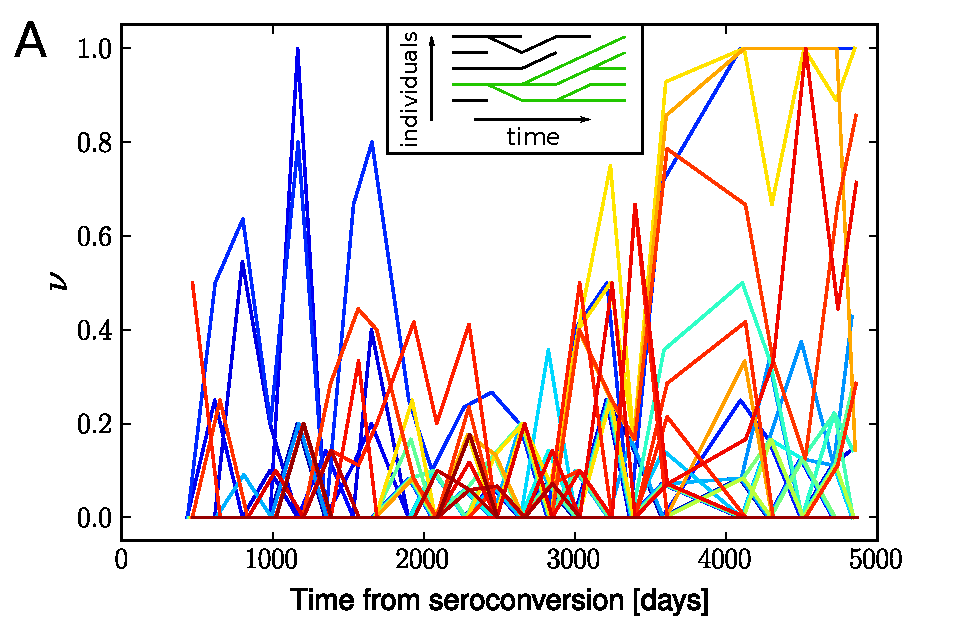
\includegraphics[width=0.6\linewidth]
{Shankarappa_allele_freqs_trajectories_syn_p10.pdf}
\label{fig:aftsyn}}\\
 \subfloat{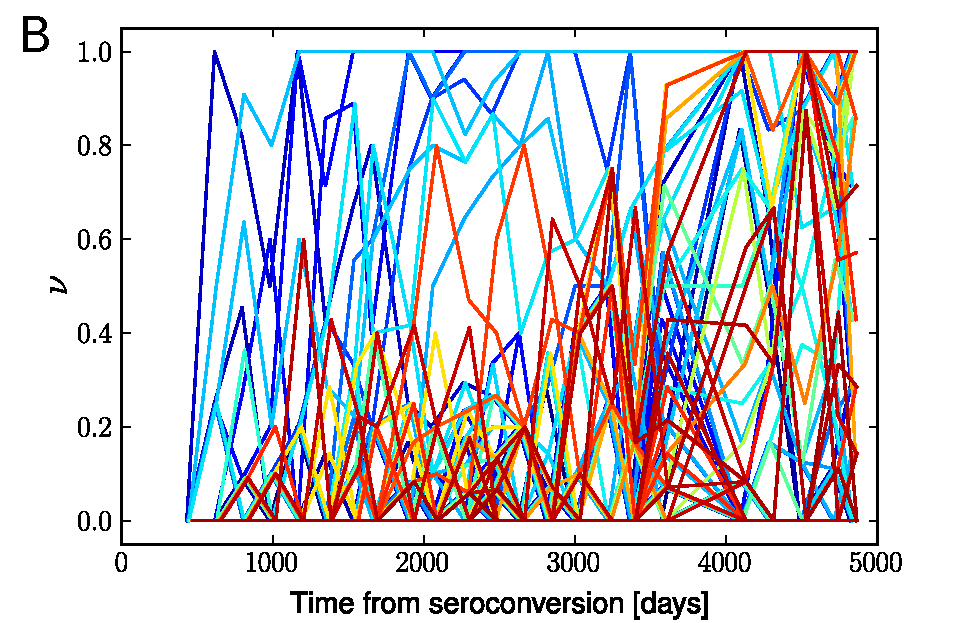
\includegraphics[width=0.6\linewidth]
{Shankarappa_allele_freqs_trajectories_nonsyn_p10.pdf}
\label{fig:aftnonsyn}}
\caption{Time series of frequencies
of synonymous (A) and nonsynonymous (B) single nucleotide variants (SNVs) in \env, 
\shankaregion, from patient p10~\cite{shankarappa_consistent_1999}.
While many nonsynonymous SNVs fix, few synonymous
SNVs do so even though they are frequently observed at high
frequencies. Colors indicate the position of the site along the \shankaregion{} region
(blue to red). Inset: the fixation probability $\pfix$ of a neutral
SNV that reached 50\% frequency is one half.}
\label{fig:aft}
\end{center}
\end{figure}


\begin{figure}
\begin{center}
\subfloat{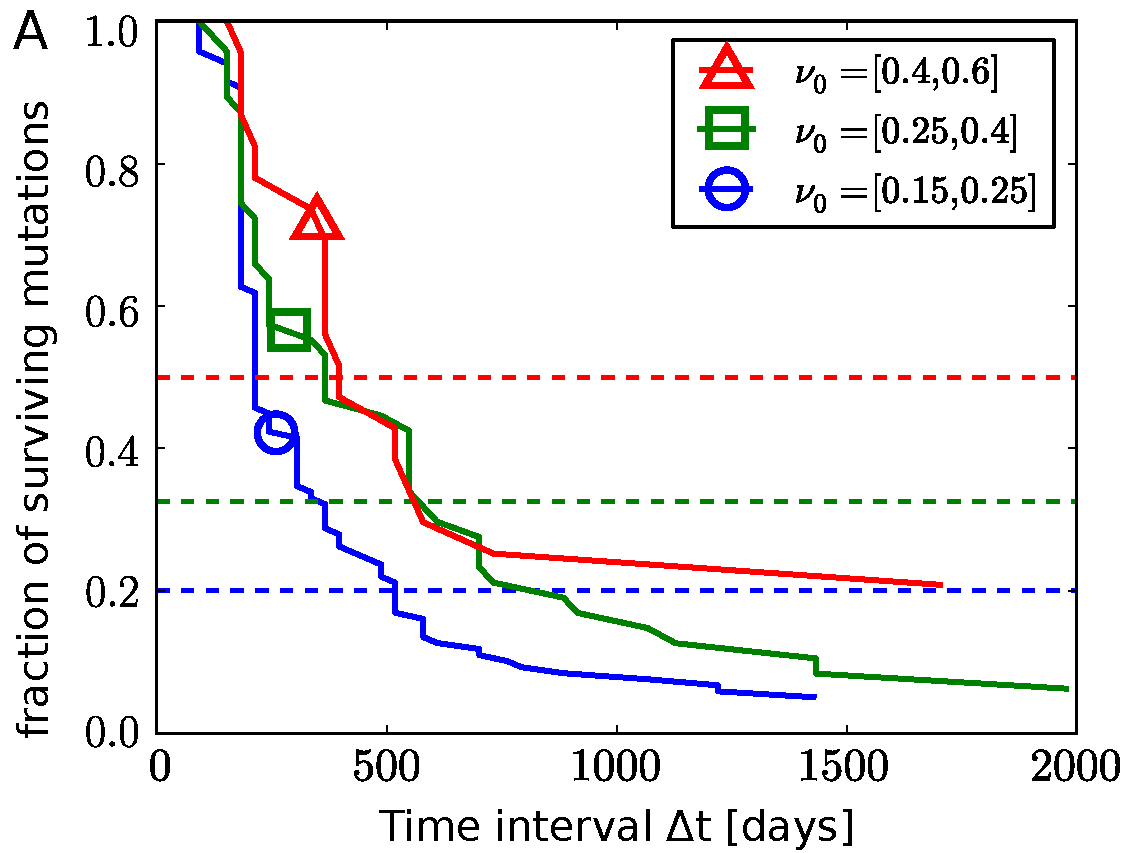
\includegraphics[width=0.6\linewidth]{fixation_times.pdf}
\label{fig:fixp1}}\\
\subfloat{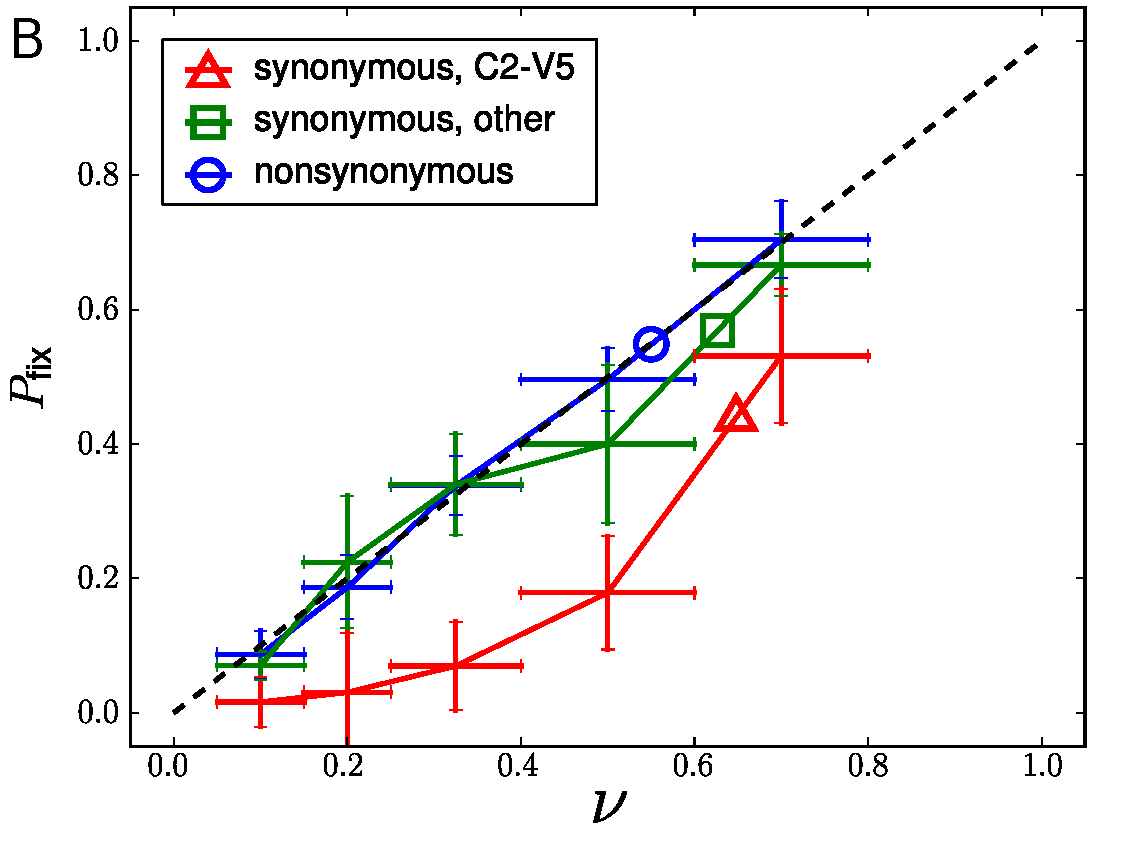
\includegraphics[width=0.6\linewidth]{fixation_probabilities.pdf}
\label{fig:fixp2}}
\caption{Fixation and loss of SNVs.
Panel A) shows how quickly synonymous SNVs are purged from the populations. 
Specifically, the figure shows the fraction of SNVs that are still observed
after $\Delta t$ days, conditional on being observed in one of the three frequency 
intervals (different colors). 
In each frequency interval, the fraction of synonymous
SNVs that ultimately survive is the fixation probability $\pfix$ conditional on the
initial frequency. The neutral expectation for $\pfix=\nu_0$ is indicated by 
dashed horizontal lines.
Panel B) shows the fixation probability of synonymous SNVs as a function of $\nu_0$. Polymorphisms within \shankaregion{} fix less
often than expected for neutral SNVs (indicated by the diagonal line).
This suppression is not observed in other parts of \env{} or for nonsynonymous
SNVs.
The horizontal error bars on the abscissa are bin sizes, the vertical ones the
standard deviation after 100 patient bootstraps of the data. Data from
refs.~\cite{shankarappa_consistent_1999,liu_selection_2006, bunnik_autologous_2008}.}
\label{fig:fixp}
\end{center}
\end{figure}

\begin{figure}
\begin{center}
\subfloat{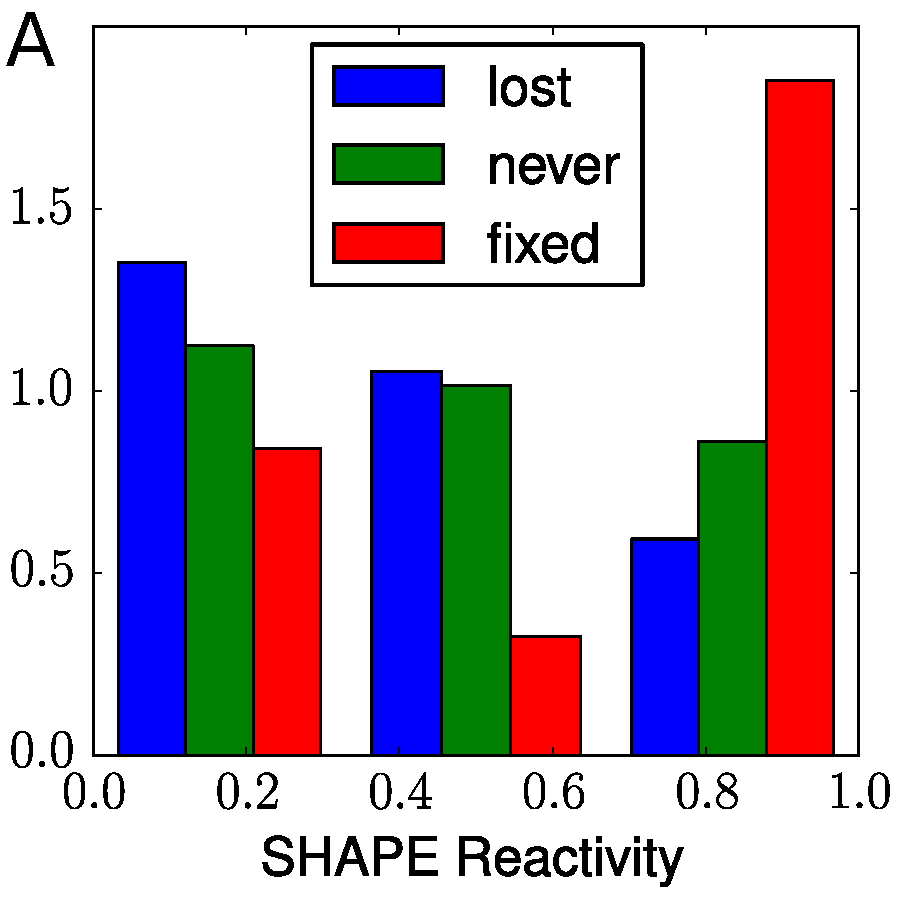
\includegraphics[height=0.3\linewidth]{reactivities_histograms_syn.pdf}\label{fig:SHAPEA}}
\subfloat{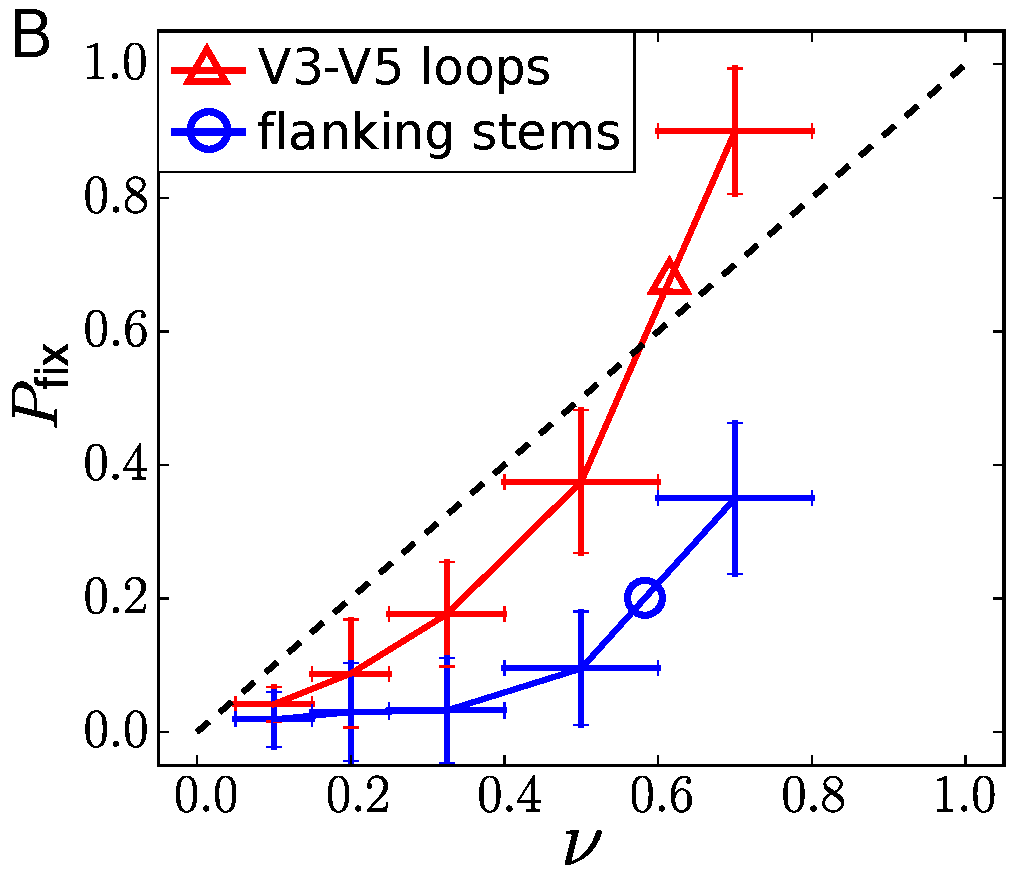
\includegraphics[height=0.3\linewidth]{fixation_probabilities_VnonV.pdf}\label{fig:SHAPEB}}
\caption{Permissible synonymous mutations tend to be unpaired.
Panel A) shows the distribution of SHAPE reactivities among sites at which synonymous 
SNVs fixed (red), sites at which SNVs reached frequencies above 15\% but
were subsequently lost (blue), and sites at which no high-frequency SNVs were observed (green) 
(all categories are restricted to the regions V1-V5$\pm 100$bp).
Sites at which SNVs fixed tend to have higher SHAPE reactivities, corresponding to
less base pairing, than those at which SNVs are lost.
Sites at which no SNVs are observed show an intermediate distribution of SHAPE values.
Panel B) shows the fixation probability of synonymous SNVs in
\shankaregion{} separately for variable regions V3-V5 and the connecting conserved 
regions C2-C4 that harbor RNA stems. As expected, the fixation probability is lower
inside the conserved regions. Data from Refs.~\cite{shankarappa_consistent_1999,
bunnik_autologous_2008, liu_selection_2006}.}
\label{fig:SHAPE}
\end{center}
\end{figure}
\begin{figure}
\begin{center}
\subfloat{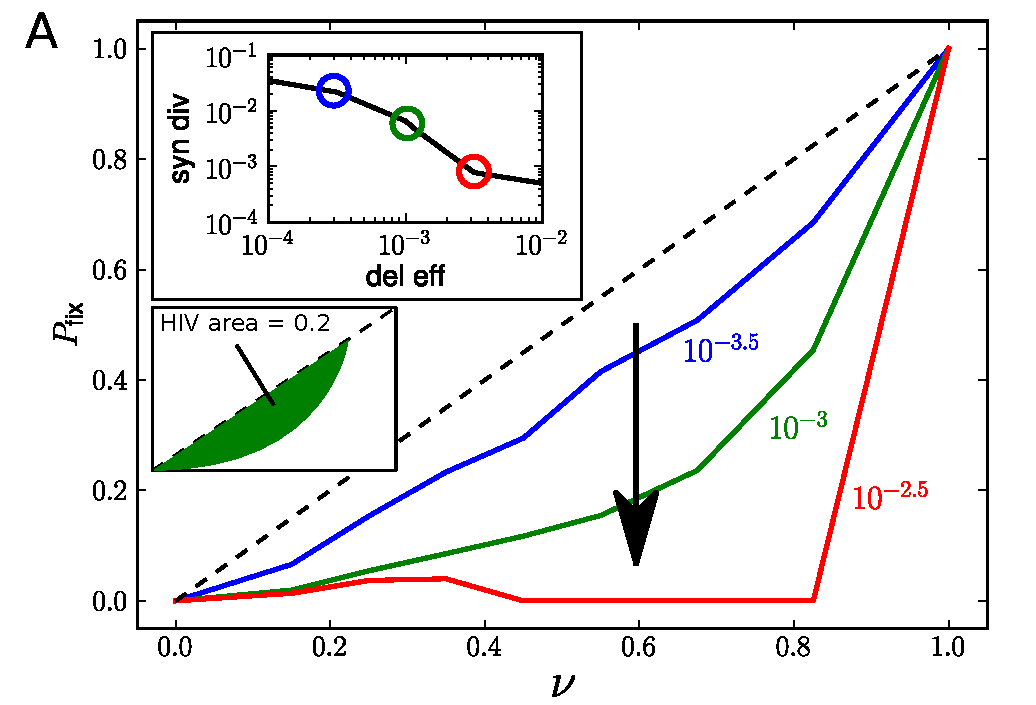
\includegraphics[width=0.6\linewidth]{simulations_graduallydel.pdf}
\label{fig:simfixpvar}}\\
\subfloat{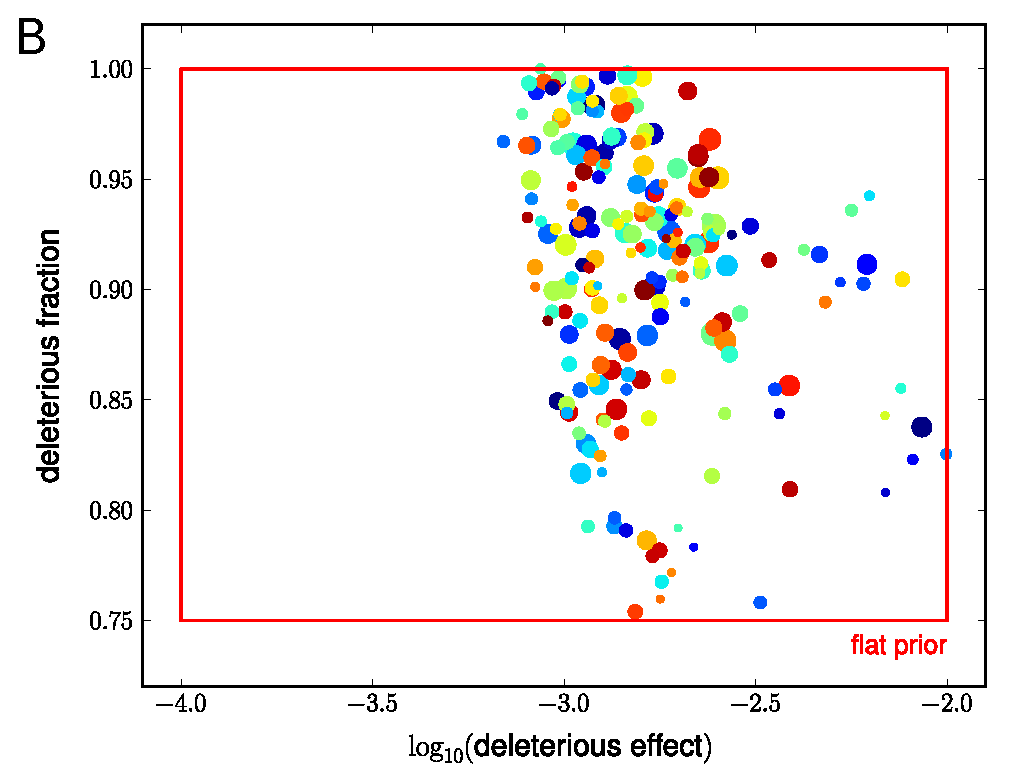
\includegraphics[width=0.6\linewidth]{simulations_syn.pdf}
\label{fig:simsfig}}
\caption{Distribution of selection coefficients on synonymous sites. Panel A)
The depression in $\pfix$ depends on the deleterious effect size 
of synonymous SNVs. This parameter also reduces synonymous
diversity, measured by the probability of a SNV to be found at
intermediate frequencies $P_\text{interm}$ (first inset).
Panel B) To assess the parameter space that affects synonymous fixation and
diversity, we run 2400 simulations with random parameters for deleterious effect
size, fraction of deleterious synonymous sites, average escape rate $\epsilon$
(color, blue to red corresponds to $10^{-2.5}$ to $10^{-1.5}$ per day), and rate of
introduction of new epitopes (marker size, from $10^{-3}$ to $10^{-2}$ per
day). Only simulations that reproduce the synonymous diversity and fixation
patterns observed in data are shown. These simulations demonstrate that
deleterious effects are around $-0.002$ and a large fraction of the 
synonymous mutations needs to be deleterious. As expected, larger
$s_d$ require larger $\epsilon$. Parameters are chosen
from prior distributions uniform in logspace as indicated by the red rectangle
(see methods).}
\label{fig:simheat}
\end{center}
\end{figure}

%\setcounter{figure}{0}
%
%%% Local Variables: 
%%% mode: latex
%%% TeX-master: t
%%% End: 

% use S1..S4 for figures numbers
\makeatletter 
\renewcommand{\thefigure}{S\@arabic\c@figure}
\makeatother

%%%%%%%%%%%%%%%%%%%%%%%%%%%%%%%%%%%%%%%%%%%%%%%%%%%%%%%%%%%%%%%%%%%%%%%%%
\section{Selection of the patient data}
%%%%%%%%%%%%%%%%%%%%%%%%%%%%%%%%%%%%%%%%%%%%%%%%%%%%%%%%%%%%%%%%%%%%%%%%%
\begin{figure}[ht]
\begin{center}
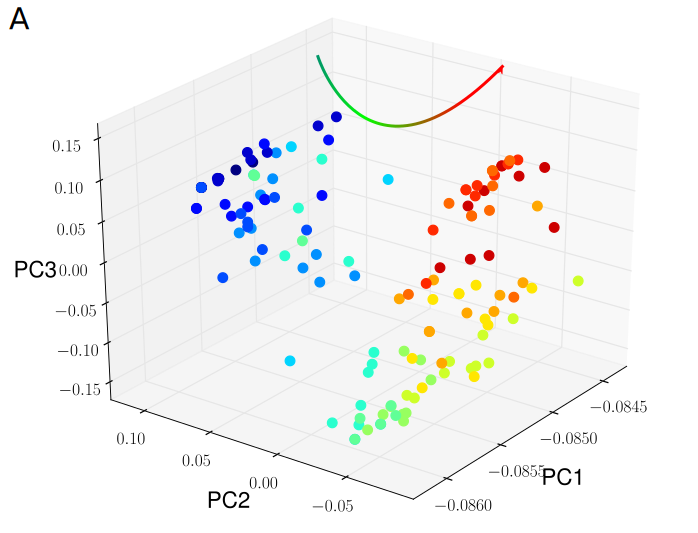
\includegraphics[width=0.35\linewidth]{Shankarappa_PCA_p1}
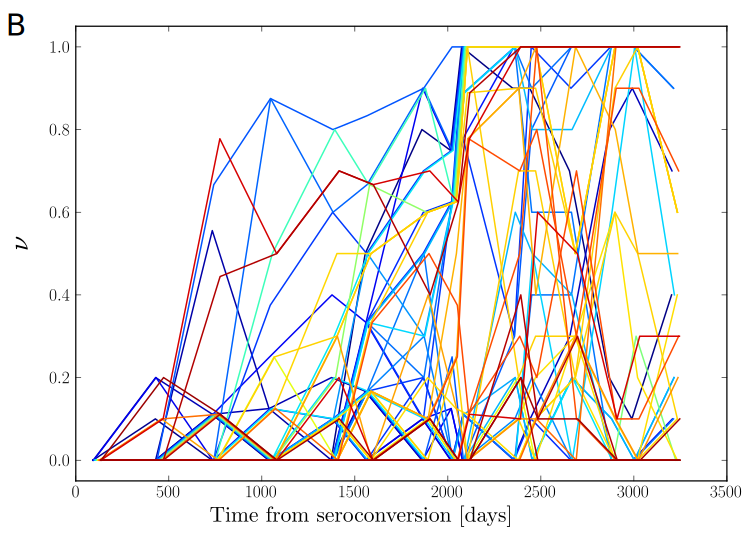
\includegraphics[width=0.35\linewidth]{Shankarappa_allele_freqs_trajectories_nonsyn_p1}
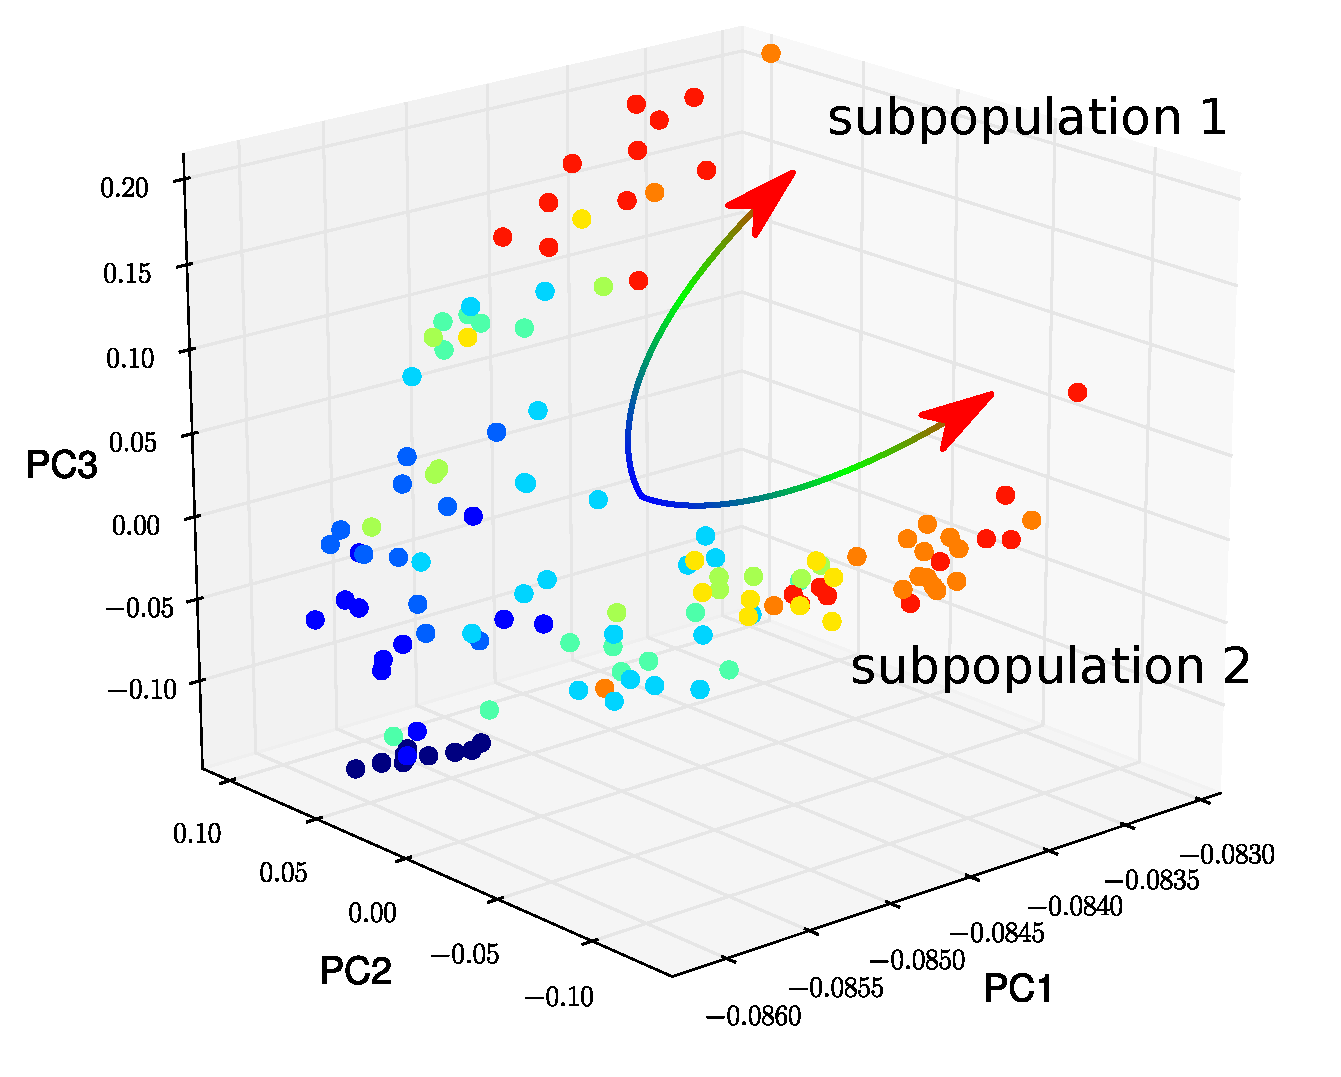
\includegraphics[width=0.35\linewidth]{Shankarappa_PCA_p7}
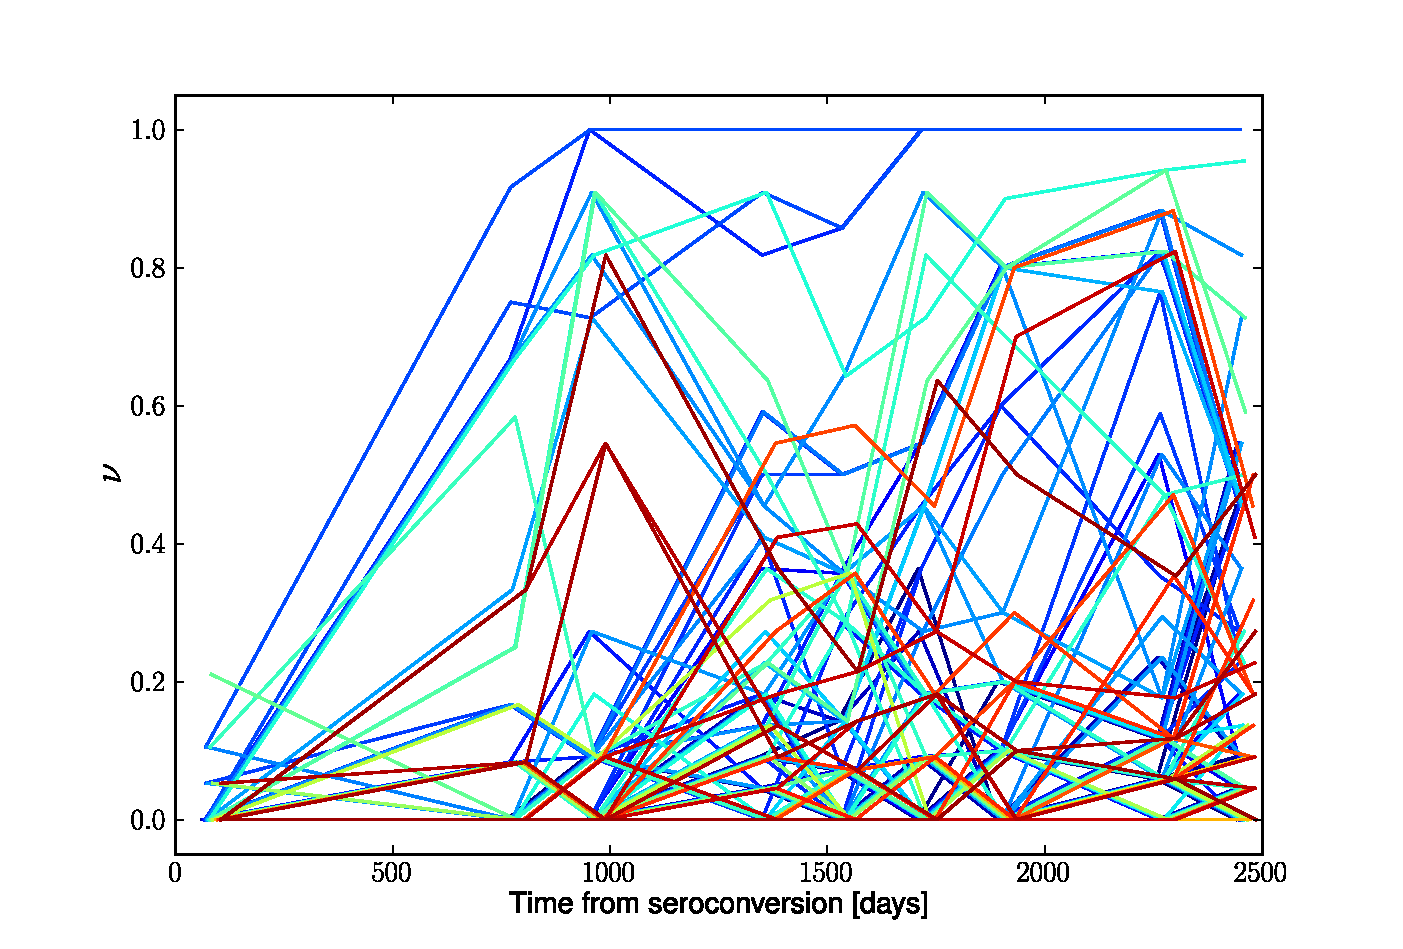
\includegraphics[width=0.35\linewidth]{Shankarappa_allele_freqs_trajectories_nonsyn_p7}
\caption{Structure of viral populations and patient selection.
Panel A) shows a PCA of all sequences from patient p1 (colors indicate time from
seroconversion, from blue to red). Panel B) shows allele frequency trajectories for nonsynonymous
changes in the same patient. Here, the blue to red color map corresponds to the
position of the allele in \env{} from 5' to 3'. Panels C) and D) show analogous
plots for data from patient p7. Samples after day 1000 split into two clusters
in the PCA and no single nucleotide variants (SNVs) that arise after day 1000 fix, presumably because they are restricted
to one subpopulation. All patients like p7 (p4, p7, p8, p9 from ref.~\citealp{shankarappa_consistent_1999} and
ACH19542 and ACH19768 from ref.~\citealp{bunnik_autologous_2008}) were excluded
from our analysis.}
\label{fig:aftp}
\end{center}
\end{figure}

\newpage
% %%%%%%%%%%%%%%%%%%%%%%%%%%%%%%%%%%%%%%%%%%%%%%%%%%%%%%%%%%%%%%%%%%%%%%%%
\section{Synonymous diversity across the HIV genome}
% %%%%%%%%%%%%%%%%%%%%%%%%%%%%%%%%%%%%%%%%%%%%%%%%%%%%%%%%%%%%%%%%%%%%%%%%
\begin{figure}[h]
\begin{center}
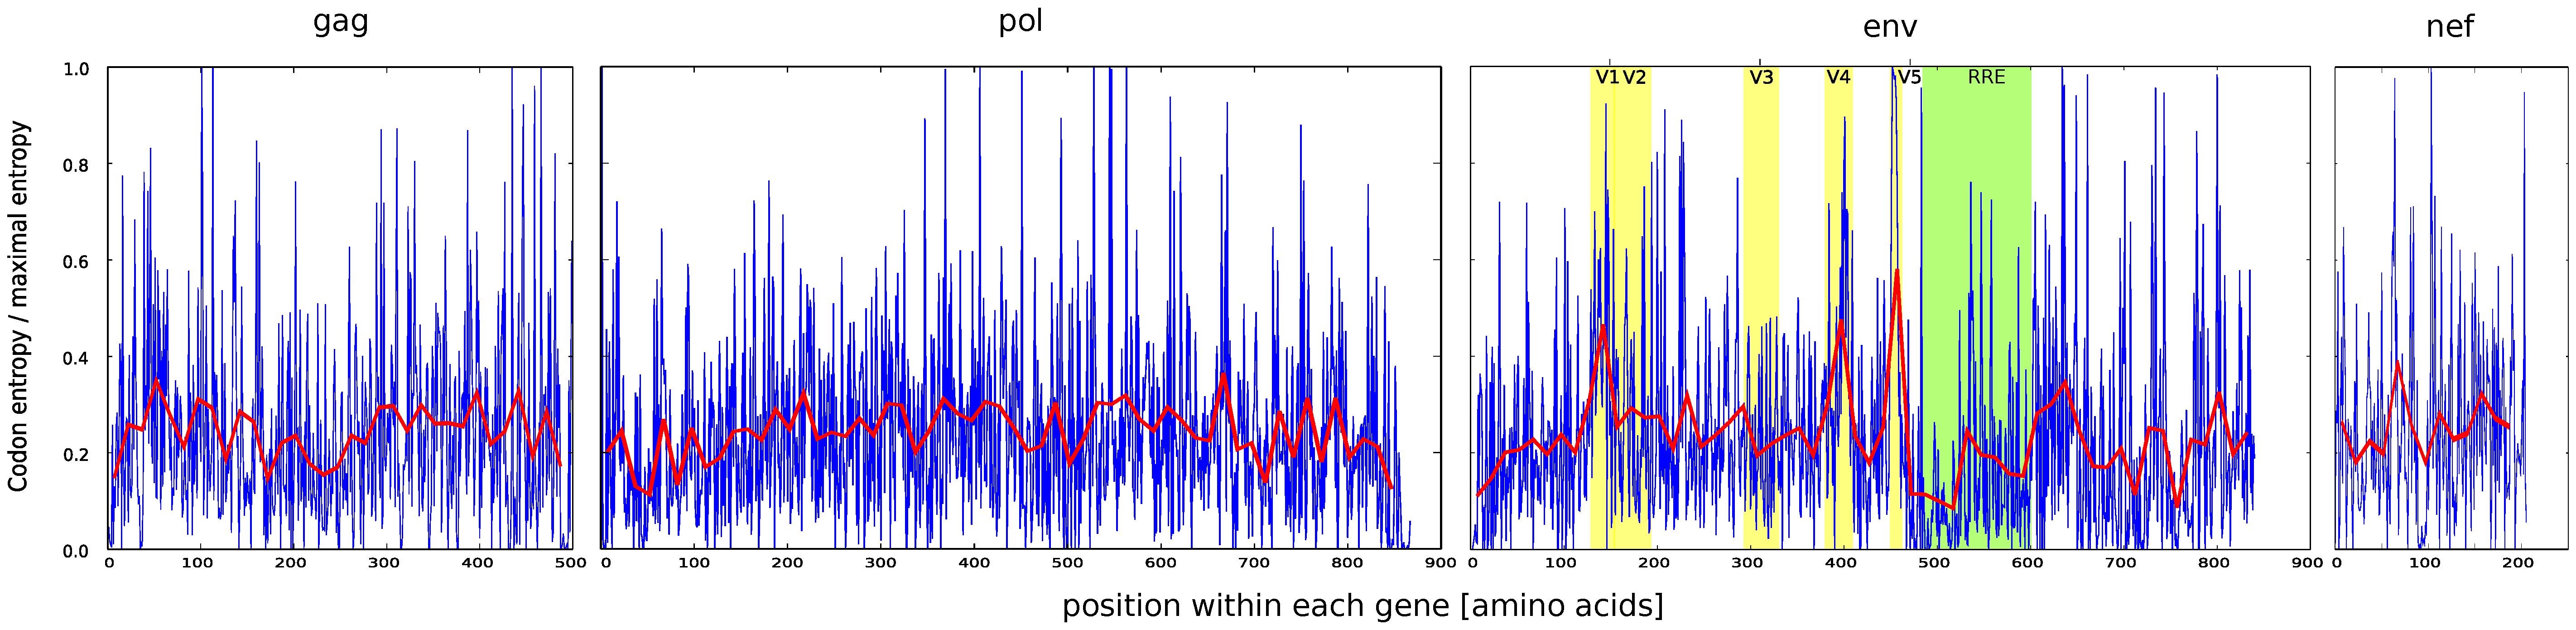
\includegraphics[width=\linewidth]{conservation_codons_genome}
\caption{
Synonymous diversity across the HIV genome, as quantified by the normalized
codon entropy among sequences coding for the consensus amino acid. In most
parts of the genome, synonymous sites show little conservation. The synonymous
diversity peaks at the variable regions in {\it env} and is reduced in regions 
under purifying selection (RRE hairpin, second {\it tat}/{\it rev} exons). The
normalized codon entropy is calculated as follows (see the script
\texttt{codon\_entropy\_synonymous\_subtypeB.py} for the full algorithm): (i)
from a subtype B multiple sequence alignment (MSA) from the LANL website (filtered sequences only, version 2011)~\cite{LANL2012}, we calculate the
consensus amino acid at each position in the HIV genome; (ii) we count how often
each codon coding for the consensus amino acid appears in the MSA; (iii) at each
amino acid position, we divide by the number of sequences in the MSA that had
the consensus amino acid at that position, obtaining {\it codon frequencies}
$\nu_c$; (iv) we calculate the codon entropy from each position as: $S := -
\sum_{c} \nu_c \log \nu_c$, where $c$ runs over codons that code for the
consensus amino acid at this site; (v) we divide by the maximal codon entropy of
that amino acid (e.g. $\log 2$ for twofold degenerate codons). All parts of
{\it env} that are part of a different gene (signaling peptide, second {\it rev}
exon) have been excluded from our main analysis, to avoid contamination by
protein selection in a different reading frame.
Note that all gap-rich columns of the MSA are stripped from this figure, so genes such as {\it env} might appear shorter than they actually
are.
}
\label{fig:syndiv_genome}
\end{center}
\end{figure}
\newpage
% 
% %%%%%%%%%%%%%%%%%%%%%%%%%%%%%%%%%%%%%%%%%%%%%%%%%%%%%%%%%%%%%%%%%%%%%%%%%
% \section{Nonsynonymous changes outside of variable regions are deleterious}
% %%%%%%%%%%%%%%%%%%%%%%%%%%%%%%%%%%%%%%%%%%%%%%%%%%%%%%%%%%%%%%%%%%%%%%%%%
% \begin{figure}[h]
% \begin{center}
% 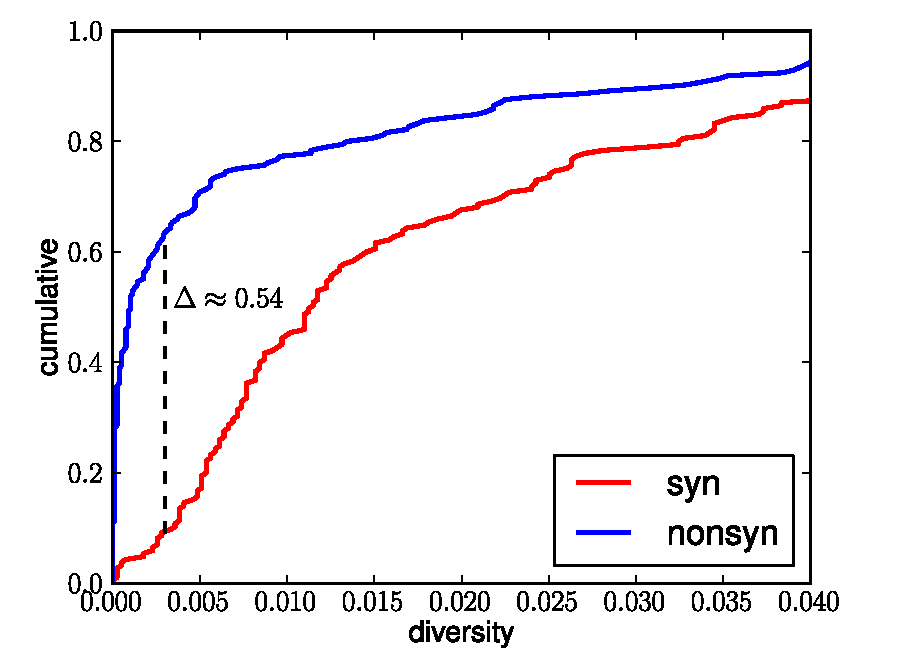
\includegraphics[width=0.8\linewidth]{synmut_conservation_4fold_synnonsyn}
% \caption{Cumulative distribution of synonymous and nonsynonymous diversity in
% {\it gag} in the LANL reference panel (filtered
% sequences only, version 2011)~\cite{LANL2012}. Sites such that the consensus codon
% has three synonymous and six nonsynonymous single mutants were used, and the number of observed mutants
% of a certain type over the number of possible mutants is plotted. Nonsynonymous
% changes are observed less often, {\it ergo} are more conserved, than
% synonymous changes. It can be therefore assumed, as mentioned in the main text,
% that non-escape nonsynonymous changes involve a large fitness cost.}
% \label{fig:synnonsyncons}
% \end{center}
% \end{figure}
% \newpage

%%%%%%%%%%%%%%%%%%%%%%%%%%%%%%%%%%%%%%%%%%%%%%%%%%%%%%%%%%%%%%%%%%%%%%%%%
\section{Time-dependent selection}
%%%%%%%%%%%%%%%%%%%%%%%%%%%%%%%%%%%%%%%%%%%%%%%%%%%%%%%%%%%%%%%%%%%%%%%%%
\begin{figure}[h]
\begin{center}
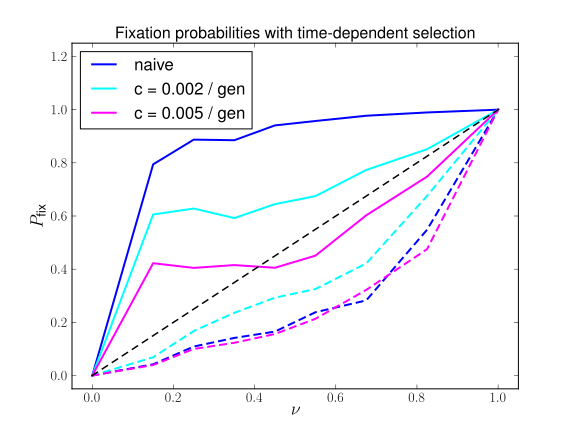
\includegraphics[width=0.6\linewidth]{simulations_gradually_timeselec_deadagain}
\caption{
Time-dependent selection reduces fixation of nonsynonymous SNVs. The figure
compares the fixation probability in the time independent model (na\"ive) to
a model with time dependent selection that mimics  an evolving immune system.
It has been found that virus is typically neutralized by serum from a few months
earlier~\citep{richman_rapid_2003} but not by contemporary serum. We model this
evolving immune system by assuming that escaped variants lose their beneficial
effect with a rate proportional to the frequency of the escaped variant. 
Specifically, the selection effect of the escape mutations is
reset to its fitness cost of $-0.02$ with probability
\[ P_\text{recognized}(t) = c \cdot \nu(t), \] 
per generation, where $c$ is a constant coefficient shown in the legend that
encodes the overall efficiency of the host immune system. With increasing
probability of recognition, the fixation of frequent escape mutants is reduced,
while hitch-hiking of synonymous SNVs is not affected. The precise
shape of $\pfix(\nu)$ depends on the details of the $P_\text{recognized}(t)$, and 
we do not think that the high $\pfix(\nu)$ for $\nu<0.2$ is meaningful.
The other parameters for the shown simulations are
the following: deleterious effect $s_d = 10^{-3}$, average escape rate $\epsilon = 0.016$,
fraction of deleterious synonymous mutations $\alpha = 0.986$, rate of new epitopes
$k_A=0.0014$ per generation.
}
\label{fig:tds}
\end{center}
\end{figure}

\newpage
%%%%%%%%%%%%%%%%%%%%%%%%%%%%%%%%%%%%%%%%%%%%%%%%%%%%%%%%%%%%%%%%%%%%%%%%%
\section{Within-epitope competition}
%%%%%%%%%%%%%%%%%%%%%%%%%%%%%%%%%%%%%%%%%%%%%%%%%%%%%%%%%%%%%%%%%%%%%%%%%
\begin{figure}[h]
\begin{center}
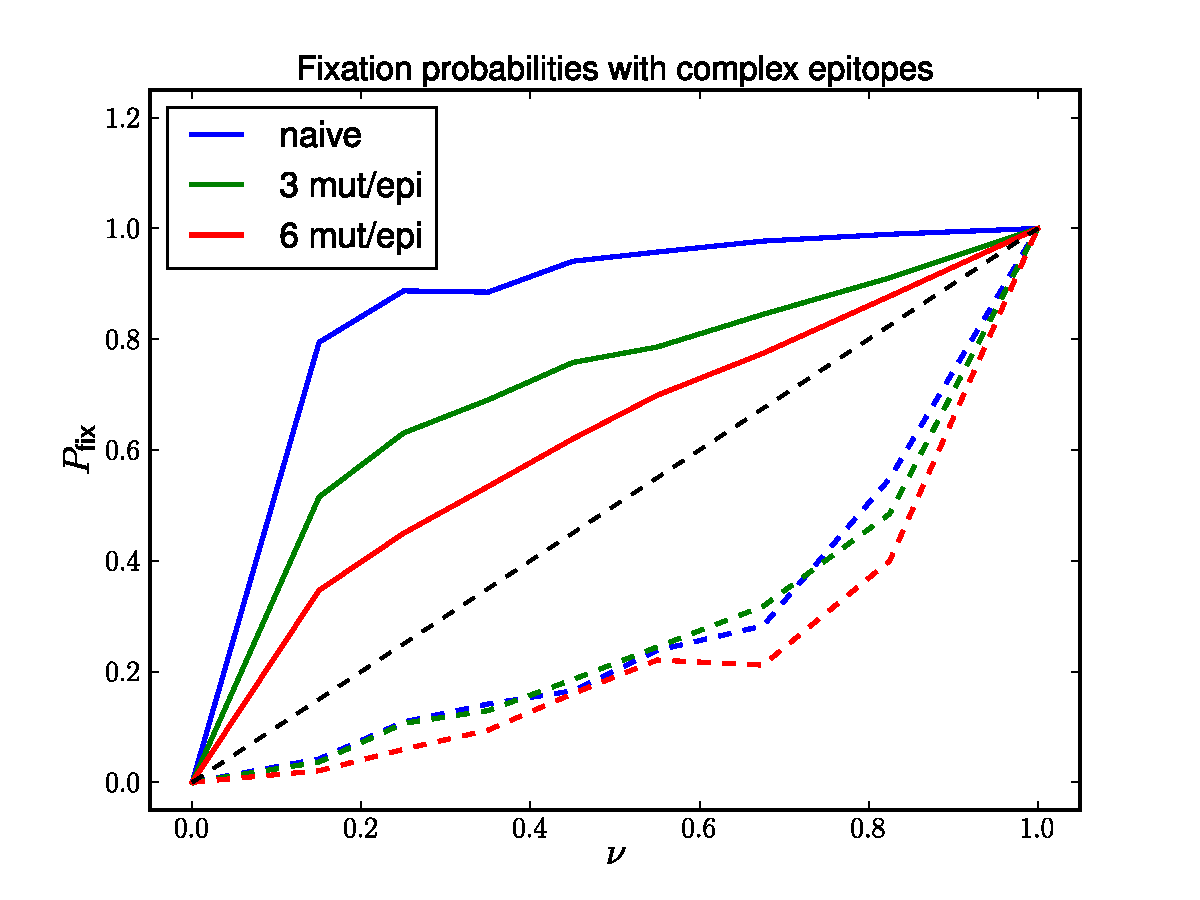
\includegraphics[width=0.6\linewidth]{simulations_gradually_epitopes}
\caption{
Competition between escape SNVs in the same epitope reduces fixation of
nonsynonymous SNVs. The figure compares the fixation probability of models
with one, three, or six mutually exclusive escape mutations within the
same epitope. Within epitope competition results in reduced fixation
probabilities of nonsynonymous changes, whereas the synonymous changes behave 
similarly in all cases. We assume that escape can happen at $n$ sites out of 3
consecutive codons and vary $n$.
The fitness landscape of each epitope includes negative epistatic terms, so that
the joint presence of more than one escape mutation is not any more beneficial
for the virus than a single mutation. Specifically, each site has two alleles,
$\pm 1$, where $-1$ is the ancestral one and $+1$ the derived one; the fitness
coefficient of a $k$-tuple of sites within the epitope is $f_k = (-1)^{k-1}
2^{1-n}\eta_\epsilon $, where $\eta_\epsilon$ is the escape rate of the epitope
drawn from an exponential distribution with mean $\epsilon$ and 
$n$ is the number of competing escapes in the epitope. 
In this evolutionary scenario, many escape SNVs start to sweep on different backgrounds within the viral population, but eventually
compete and only one of them fixes. The other parameters for the shown simulations are
the following: deleterious effect $s_d = 10^{-3}$, average escape rate $\epsilon = 0.016$,
fraction of deleterious synonymous mutations $\alpha = 0.986$, rate of new epitopes
$k_A=0.0014$ per generation.
}
\label{fig:wec}
\end{center}
\end{figure}

%%%%%%%%%%%%%%%%%%%%%%%%%%%%%%%%%%%%%%%%%%%%%%%%%%%%%%%%%%%%%%%%%%%%%%%%%
\end{document}
%%%%%%%%%%%%%%%%%%%%%%%%%%%%%%%%%%%%%%%%%%%%%%%%%%%%%%%%%%%%%%%%%%%%%%%%%
